% Made up for the tikra gallery: the normal curve, its mean and its spread. In the playground,
% drag the top of the curve: sideways moves the mean, up and down changes the spread.
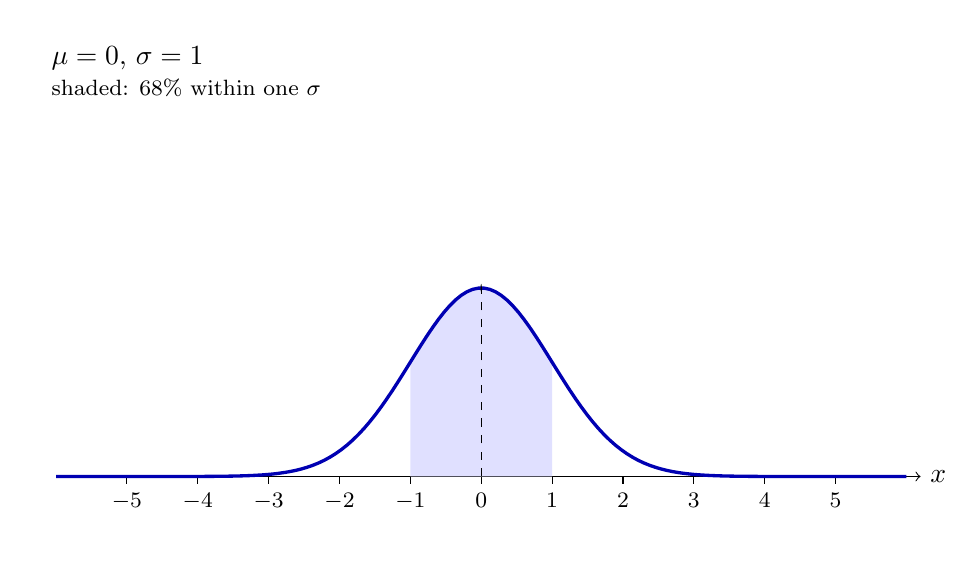
\begin{tikzpicture}[xscale=0.9, yscale=6]
  \def\m{0}      % mean, -3..3
  \def\s{1}      % standard deviation, 0.5..2.5
  \useasboundingbox (-6.4,-0.12) rectangle (6.4,0.95);
  \draw[->] (-6,0) -- (6.2,0) node[right] {$x$};
  \foreach \x in {-5,...,5} \draw (\x,0) -- (\x,-0.015) node[below] {\footnotesize $\x$};
  \fill[blue!12, domain={\m-\s}:{\m+\s}, samples=60] (\m-\s,0) -- plot (\x, {exp(-(\x-\m)^2/(2*\s^2))/(\s*sqrt(2*pi))}) -- (\m+\s,0) -- cycle;
  \draw[very thick, blue!70!black, domain=-6:6, samples=150] plot (\x, {exp(-(\x-\m)^2/(2*\s^2))/(\s*sqrt(2*pi))});
  \coordinate (top) at (\m, {1/(\s*sqrt(2*pi))});
  \draw[dashed] (\m,0) -- (top);
  \fill (top) circle (0.25pt);
  \node[anchor=north west, align=left] at (-6.2,0.93) {$\mu = \pgfmathprintnumber[fixed, precision=2]{\m}$, $\sigma = \pgfmathprintnumber[fixed, precision=2]{\s}$\\[-1pt]
    \footnotesize shaded: $68\%$ within one $\sigma$};
\end{tikzpicture}
